\begin{example}[3]Helicoid and catenoid (from homework)

In your homework you have found local parametrization of helicoid and 
catenoid 
\begin{align*}
    H(u,v)&=\left(v\cos u, v\sin u, a u\right)\\
    C(\varphi,\theta)&=\left(a \cosh \theta \cos \varphi,
    a\cosh \theta \sin \varphi ,a \theta \right) .       
\end{align*}
\begin{figure}[h]
    \centering
    \begin{subfigure}{0.3\textwidth}
        \centering
        \includegraphics[scale=0.65]{picture/week7/helicoid.png}
        \caption{Helicoid}
    \end{subfigure}
    \begin{subfigure}{0.3\textwidth}
        \centering
        \includegraphics[scale=1.5]{picture/week7/catenoid.png}
        \caption{Catenoid}    
    \end{subfigure}
\end{figure}
\begin{enumerate}[(1)]
    \item Compute the \engordnumber{1} fundamental form of them.
    \[ I_H=\left(v^2+a^2\right)\dd u^2+\dd v^2\]
    \[I_C=\left(a^2\cosh^2\theta\right)\dd\varphi^2+
    \left(a^2\cosh^2\theta\right)\dd \theta^2\]
    \item Show that there is a parametrization on the helicoid, 
    \(\tilde{H}\left(\tilde{u},\tilde{v}\right)\), such that
    \[
        I_{\tilde{H}}=\left(a^2\cosh^2\tilde{v}\right)\dd \tilde{u}^2
        +\left(a^2\cosh^2\tilde{v}^2\right)\dd \tilde{v}^2    
    .\]
    (\(u=\tilde{u},v=a\sinh\tilde{v}\))
\end{enumerate}
\end{example}
\begin{remark}
    In both example 1 and example 3, we have seen that near a point, 
    the two surfaces considered have the same \engordnumber{1} 
    fundamental form
     (after a change of parametrization). Such property is called
      ``local isometry''. We'll make this definition more clear later.
\end{remark}

\(\bullet\)Application of the \engordnumber{1} fundamental form

\begin{enumerate}[(1)]
    \item Arclength of a curve on \(S\)
    Note that for a vector \(v\in \mathbb{R}^2\), \(I(v,v)=|v|^2\).
    Let \(\alpha(t)\colon (0,t)\to S\) be a curve in \(S\) and 
    \(\varphi \colon U\to S\), \((u,v)\mapsto\varphi (u,v)\) be a 
    local parametrization satisfying 
    \(\alpha(t)\in \varphi(U)\).
    \[
    \Rightarrow \alpha(t)=\varphi\left(u(t),v(t)\right) .   
    \]
    \[
      \Rightarrow\alpha'(t)=\varphi_u u'(t)+\varphi_v v'(t) .
    \]
    \[\Rightarrow \left|\alpha'(t)\right|^2=
    I\left(\alpha'(t),\alpha'(t)\right)=E u_t^2+2F u_t v_t +G v_t^2.\]
    The arclength of \(\alpha(t)\) is defined by 
    \[
        s(t)=\int_0^t  \left|\alpha'(t)\right|\dd t
        =\int_0^t \sqrt{E u_t^2+2F u_t v_t +G v_t^2}\dd t  .
    \]
    \[
        \Rightarrow \dd s=\sqrt{E u_t^2+2F u_t v_t +G v_t^2}\dd t.
    \]
    \[
        \Rightarrow\left(\dv{s}{t}\right)^2=E u_t^2+2F u_t v_t +G v_t^2.
    \]
    \[
        \Rightarrow \dd s^2=E \dd u^2+2F \dd u \dd v +G \dd v^2    .
    \]
    This explains the ``geometric meaning'' of \(I\), \ie\ it measures 
    the infinitesimal arclength.
    \item Angle between two curves intersecting at \(t_0\)
    Let \(\alpha\colon I\to S\), \(\beta\colon I\to S\) be two curves 
    on \(S\), \(\alpha(t_0)=\beta(\bar{t}_0)=p\in S\). 
    \begin{center}
        


\tikzset{every picture/.style={line width=0.75pt}} %set default line width to 0.75pt        

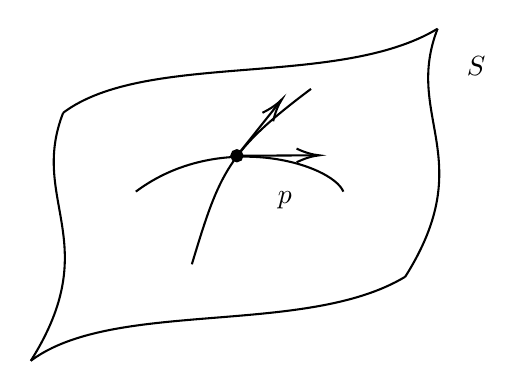
\begin{tikzpicture}[x=0.75pt,y=0.75pt,yscale=-1,xscale=1]
%uncomment if require: \path (0,300); %set diagram left start at 0, and has height of 300

%Curve Lines [id:da9909335153566519] 
\draw    (183,147) .. controls (223,117) and (315.4,135.5) .. (363.4,106.5) ;
%Curve Lines [id:da019275275220669075] 
\draw    (167.4,266.5) .. controls (203.4,209.5) and (166.4,189.5) .. (183,147) ;
%Curve Lines [id:da6995475257546488] 
\draw    (167.4,266.5) .. controls (207.4,236.5) and (299.8,255) .. (347.8,226) ;
%Curve Lines [id:da33316817877336646] 
\draw    (347.8,226) .. controls (383.8,169) and (346.8,149) .. (363.4,106.5) ;
%Shape: Circle [id:dp7349369009552857] 
\draw  [fill={rgb, 255:red, 0; green, 0; blue, 0 }  ,fill opacity=1 ] (264,167.7) .. controls (264,166.21) and (265.21,165) .. (266.7,165) .. controls (268.19,165) and (269.4,166.21) .. (269.4,167.7) .. controls (269.4,169.19) and (268.19,170.4) .. (266.7,170.4) .. controls (265.21,170.4) and (264,169.19) .. (264,167.7) -- cycle ;
%Curve Lines [id:da09382061994840107] 
\draw    (218,185) .. controls (258,155) and (312.4,171.5) .. (318,185) ;
%Curve Lines [id:da6577705388758515] 
\draw    (245,220) .. controls (258.4,175.5) and (262.4,165.5) .. (302.4,135.5) ;
%Straight Lines [id:da2459893691777446] 
\draw    (266.7,167.7) -- (287.15,142.06) ;
\draw [shift={(288.4,140.5)}, rotate = 128.58] [color={rgb, 255:red, 0; green, 0; blue, 0 }  ][line width=0.75]    (10.93,-3.29) .. controls (6.95,-1.4) and (3.31,-0.3) .. (0,0) .. controls (3.31,0.3) and (6.95,1.4) .. (10.93,3.29)   ;
%Straight Lines [id:da2821040919294362] 
\draw    (266.7,167.7) -- (304.4,167.51) ;
\draw [shift={(306.4,167.5)}, rotate = 179.71] [color={rgb, 255:red, 0; green, 0; blue, 0 }  ][line width=0.75]    (10.93,-3.29) .. controls (6.95,-1.4) and (3.31,-0.3) .. (0,0) .. controls (3.31,0.3) and (6.95,1.4) .. (10.93,3.29)   ;

% Text Node
\draw (376,118.4) node [anchor=north west][inner sep=0.75pt]    {$S$};
% Text Node
\draw (285,183.4) node [anchor=north west][inner sep=0.75pt]    {$p$};


\end{tikzpicture}
    \end{center}
    Define
        \[
            \cos \theta=\frac{\left\langle\alpha'(t_0),
            \beta'(\bar{t}_0)\right\rangle_{\mathbb{R}^3}}{
            \left|\alpha'(t_0)\right|\left|\beta'(\bar{t}_0) \right|}.
        \]
    \begin{question}
        Given a parametrization \(\varphi(u,v)\),
         we have two coordinate
         curve \(\varphi(u,v_0)\), \(\varphi(u_0,v)\). What's the angle 
         between them?
         \[u\text{-curve: }\alpha(t)=\varphi\left(u(t),c\right)
         \Rightarrow \alpha'(t)=\varphi_u u'.\]
         \[v\text{-curve: }\beta(t)=\varphi\left(c,v(t)\right)
         \Rightarrow \beta'(t)=\varphi_v v'.\] 
         \[
            \Rightarrow \cos \theta= 
            \frac{\left\langle \varphi_u u',\varphi_v v'\right\rangle}{
                \left|\varphi_u u'\right|\left|\varphi_v v'\right|
            }
            =\pm \frac{\left\langle\varphi_u,\varphi_v
            \right\rangle_{\mathbb{R}^3}}{\left|\varphi_u\right|
            \left|\varphi_v\right|}=\pm \frac{F}{\sqrt{EG}}  
         .\]
         In particular, we conclude that
         \[F=0\Leftrightarrow \text{Two coordinate curves are orthogonal,}\]
         and such parametrization is called an orthogonal parametrization.
         (e.g. \(\mathbb{S}^2\), \(\theta,\varphi\) and stereographic
          projection are two such parametrizations) 
    \end{question}
    \item (Surface) area
    Let \(S\) be a regular surface. Choose a parametrization 
    \(\varphi\colon U\to S\). Let \(Q\subset S\) be a bounded domain.
    Assume \(Q\subset \varphi(U)\), so \(\varphi^{-1}(Q)\subset U\) is 
    a bounded set in \(\mathbb{R}^2\).
    \begin{center}
\tikzset{every picture/.style={line width=0.75pt}} %set default line width to 0.75pt        

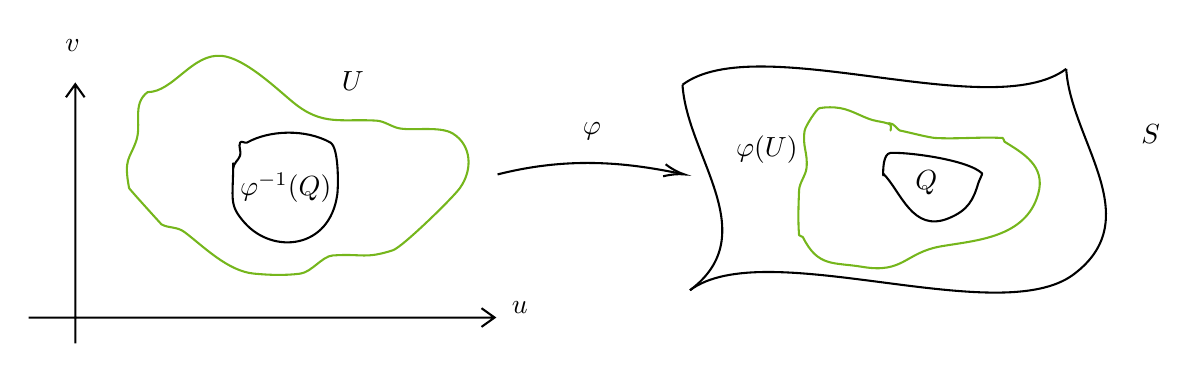
\begin{tikzpicture}[x=0.75pt,y=0.75pt,yscale=-0.9,xscale=0.9]
%uncomment if require: \path (0,300); %set diagram left start at 0, and has height of 300

%Shape: Axis 2D [id:dp30826843172023066] 
\draw  (67,239.62) -- (316.4,239.62)(91.94,114.71) -- (91.94,253.5) (309.4,234.62) -- (316.4,239.62) -- (309.4,244.62) (86.94,121.71) -- (91.94,114.71) -- (96.94,121.71)  ;
%Curve Lines [id:da2230443220096674] 
\draw [color={rgb, 255:red, 117; green, 182; blue, 28 }  ,draw opacity=1 ][line width=0.75] [line join = round][line cap = round]   (130.65,118.95) .. controls (122.05,125.38) and (127.75,136.1) .. (124.46,145.32) .. controls (121.04,154.89) and (117.73,154.56) .. (120.74,170.31) .. controls (120.84,170.81) and (138.01,189.7) .. (138.08,189.74) .. controls (142.04,191.95) and (146.26,190.76) .. (150.46,193.9) .. controls (160.22,201.19) and (173.4,214.78) .. (187.61,216.11) .. controls (195.84,216.88) and (204.18,217.17) .. (212.38,216.11) .. controls (218.48,215.32) and (224.1,206.79) .. (229.72,206.39) .. controls (245.72,205.27) and (246.88,208.43) .. (261.91,203.62) .. controls (267,201.99) and (294.17,175.43) .. (297.82,170.31) .. controls (304.87,160.44) and (304.12,147.39) .. (294.11,141.16) .. controls (287.42,136.99) and (273.12,139.67) .. (265.63,138.38) .. controls (261.37,137.65) and (257.55,134.47) .. (253.25,134.22) .. controls (234.05,133.09) and (224.32,137.27) .. (208.67,124.5) .. controls (200.24,117.64) and (182.83,100.69) .. (170.28,99.52) .. controls (154.41,98.04) and (144.45,118.95) .. (130.65,118.95) -- cycle ;
%Curve Lines [id:da779384228982472] 
\draw [line width=0.75] [line join = round][line cap = round]   (176.47,157.04) .. controls (176.47,176.42) and (173.86,179.1) .. (182.66,188.96) .. controls (197.74,205.87) and (228.15,203.16) .. (232.19,173.69) .. controls (232.75,169.62) and (233.14,148.55) .. (228.48,145.93) .. controls (215.25,138.52) and (195.8,139.26) .. (183.9,145.93) .. controls (182.79,146.56) and (180.82,144.74) .. (180.18,145.93) .. controls (179.12,147.92) and (180.91,150.71) .. (180.18,152.87) .. controls (179.34,155.4) and (176.47,157.12) .. (176.47,159.81) ;
%Curve Lines [id:da4093176006038537] 
\draw    (417,115) .. controls (457,85) and (582.4,136.5) .. (622.4,106.5) ;
%Curve Lines [id:da8843839986108935] 
\draw    (421,225) .. controls (461,195) and (586.4,246.5) .. (626.4,216.5) ;
%Curve Lines [id:da3854765584435005] 
\draw    (421,225) .. controls (461,195) and (419.4,153.5) .. (417,115) ;
%Curve Lines [id:da6146348531460317] 
\draw    (626.4,216.5) .. controls (666.4,186.5) and (624.8,145) .. (622.4,106.5) ;
%Curve Lines [id:da8543149552748068] 
\draw [color={rgb, 255:red, 117; green, 182; blue, 28 }  ,draw opacity=1 ][line width=0.75] [line join = round][line cap = round]   (528.4,139.5) .. controls (528.4,138.5) and (528.85,137.39) .. (528.4,136.5) .. controls (527.93,135.57) and (522.09,134.61) .. (521.4,134.5) .. controls (514.38,133.33) and (508.52,128.69) .. (501.4,127.5) .. controls (497.78,126.9) and (494.02,126.9) .. (490.4,127.5) .. controls (488.74,127.78) and (482.76,137.32) .. (482.4,139.5) .. controls (480.99,147.95) and (484.21,151.37) .. (483.4,159.5) .. controls (483,163.53) and (479.56,167.46) .. (479.4,171.5) .. controls (479.09,179.49) and (478.76,187.53) .. (479.4,195.5) .. controls (479.46,196.24) and (481.07,195.83) .. (481.4,196.5) .. controls (489.58,212.86) and (497.61,209.87) .. (513.4,212.5) .. controls (535.53,216.19) and (535.97,204.88) .. (555.4,201.5) .. controls (574.04,198.26) and (600.67,197.05) .. (607.4,173.5) .. controls (611.7,158.44) and (599.25,151.66) .. (589.4,145.5) .. controls (588.77,145.1) and (589.14,143.54) .. (588.4,143.5) .. controls (576.42,142.85) and (564.38,144.11) .. (552.4,143.5) .. controls (548.93,143.32) and (537.92,140.4) .. (533.4,139.5) .. controls (532.08,139.24) and (530.49,135.5) .. (527.4,135.5) ;
%Curve Lines [id:da5437419917187927] 
\draw [line width=0.75] [line join = round][line cap = round]   (524.4,162.5) .. controls (533.93,172.03) and (540,194.41) .. (559.4,186.5) .. controls (570.03,182.17) and (572.69,176.55) .. (575.4,167.5) .. controls (575.66,166.65) and (577.6,162.7) .. (577.4,162.5) .. controls (570.13,155.23) and (537.95,150.97) .. (528.4,151.5) .. controls (524.33,151.73) and (524.4,160.76) .. (524.4,163.5) ;
%Curve Lines [id:da9563040601689965] 
\draw    (318,163) .. controls (358.57,152.71) and (390.12,157.31) .. (416.4,162.67) ;
\draw [shift={(418,163)}, rotate = 191.68] [color={rgb, 255:red, 0; green, 0; blue, 0 }  ][line width=0.75]    (10.93,-3.29) .. controls (6.95,-1.4) and (3.31,-0.3) .. (0,0) .. controls (3.31,0.3) and (6.95,1.4) .. (10.93,3.29)   ;

% Text Node
\draw (178.47,160.44) node [anchor=north west][inner sep=0.75pt]    {$\varphi ^{-1}( Q)$};
% Text Node
\draw (233,106.4) node [anchor=north west][inner sep=0.75pt]    {$U$};
% Text Node
\draw (540,159.4) node [anchor=north west][inner sep=0.75pt]    {$Q$};
% Text Node
\draw (444,140.4) node [anchor=north west][inner sep=0.75pt]    {$\varphi ( U)$};
% Text Node
\draw (661,134.4) node [anchor=north west][inner sep=0.75pt]    {$S$};
% Text Node
\draw (362,133.4) node [anchor=north west][inner sep=0.75pt]    {$\varphi $};
% Text Node
\draw (324,229.4) node [anchor=north west][inner sep=0.75pt]    {$u$};
% Text Node
\draw (85,89.4) node [anchor=north west][inner sep=0.75pt]    {$v$};


\end{tikzpicture}
    \end{center}
    Let's assume the boundary of \(Q\) is a differentiable curve with 
    singularities lying in a measure zero set.
\begin{definition}[Area of \(Q\)]
    \[Area(Q)=\iint_{\varphi(Q)} \left|\varphi_u\wedge 
    \varphi_v \right|\dd u\dd v \quad(\text{double integral in }
    \mathbb{R}^2).\]
    Here, we give the definition in terms of a ``parametrization''. 
    However, the area of \(Q\) is a number only depending on \(Q\)
    itself. We should check that our definition does not depend on 
    the parametrization.
\end{definition}
\textbf{Claim}: 
\textcolor{blue}{\(Area(Q)\) defined above is independent of the
choice of parametrizations.}
\begin{proof}(Left as an excercise or homework)
    Let \(\psi(\alpha,\beta)\colon V\to S\) be another parametrization. 
    Let \(H=\psi^{-1}\circ \varphi\) be the change of parametrization,
    \(H(u,v)=(\alpha,\beta)\)\(\Rightarrow\varphi =\psi \circ H\).
    We compute \(\iint_{\varphi(Q)} \left|\varphi_u\wedge 
    \varphi_v \right|\dd u\dd v\).

    By chain rule 
    \[
        \begin{pmatrix}
            \varphi_u\\ \varphi_v
        \end{pmatrix}=
        \pdv{(\alpha,\beta)}{(u,v)}\begin{pmatrix}
            \psi_\alpha\\
            \psi_\beta
        \end{pmatrix}    .
    \]
    \begin{align*}
        \Rightarrow \varphi_u\wedge\varphi_v&=
        \left(\alpha_u\beta_v\right)\psi_\alpha\wedge\psi_\beta+
        \left(\alpha_v\beta_u\right)\psi_\beta\wedge\psi_\alpha\\
        &=\left(\alpha_u\beta_v-\alpha_v\beta_u\right)
        \psi_\alpha\wedge\psi_\beta\\
        &=\det\left(\pdv{(\alpha,\beta)}{(u,v)}\right)
        \psi_\alpha\wedge\psi_\beta.
    \end{align*}
    \[\Rightarrow \left|
        \varphi_u\wedge \varphi_v 
    \right|=\left|\det\left(\pdv{(\alpha,\beta)}{(u,v)}\right)\right|
    \left|\psi_\alpha\wedge\psi_\beta\right|.\]
    
    On the other hand,
    \[
        \begin{pmatrix}
            \dd u\\ \dd v
        \end{pmatrix}
        =\pdv{(u,v)}{(\alpha,\beta)}\begin{pmatrix}
            \dd \alpha\\
            \dd \beta
        \end{pmatrix} .
    \]
    Thus, the change of infinitesimal area element is
    \[
        \dd u\dd v=\left|\dd u\wedge\dd v\right|=
        \left|\det \left(\pdv{(u,v)}{(\alpha,\beta)}\right)\right|
        \left|\dd\alpha\wedge\dd\beta\right|=
        \left|\det \left(\pdv{(u,v)}{(\alpha,\beta)}\right)\right|
        \dd\alpha\dd\beta.
    \]
    \[\Rightarrow \left|\varphi_u\wedge \varphi_v \right|
        \dd u\dd v=\left|\psi_\alpha\wedge\psi_\beta\right|\dd \alpha
        \dd \beta.
    \]
    \[\Rightarrow \iint \left|\varphi_u\wedge \varphi_v \right|
    \dd u\dd v=\iint \left|\psi_\alpha\wedge\psi_\beta\right|\dd \alpha
    \dd \beta.\]
\end{proof}
\begin{remark}
    By the \engordnumber{1} fundamental form 
    \[
        I=E(\dd u)^2+2F \dd u\dd v+G(\dd v)^2    
    \]
    \[\Rightarrow Area=\iint \left|\varphi_u\wedge \varphi_v \right|
    \dd u\dd v=\iint \sqrt{EG-F^2}\dd u\dd v.\]
\end{remark}
\end{enumerate}
\section{Gauss map and the \engordnumber{2} fundamental form}
\(\bullet\) Gauss maps.
\begin{question}
    \textcolor{blue}{How is a regular surface curved in \(\mathbb{R}^3\)}? 
\end{question}
\underline{\textbf{Recall}}: \(S\subset\mathbb{R}^3\) is an oriented
regular surface. 
\(\Rightarrow\) We can choose a unit vector field 
    \begin{align*}
        \vb{n}\colon S&\to \mathbb{S}^2(1)\\
        p&\mapsto \vb{n}_p,
    \end{align*}
is well-defined everywhere on \(S\). Moreover, \(\vb{n}\) is a
differentiable map with its image lying on the unit sphere, and we 
called the map to be the Gauss map. \(\vb{n}\) determines an 
orientation of \(S\).
\begin{center}
    


\tikzset{every picture/.style={line width=0.75pt}} %set default line width to 0.75pt        

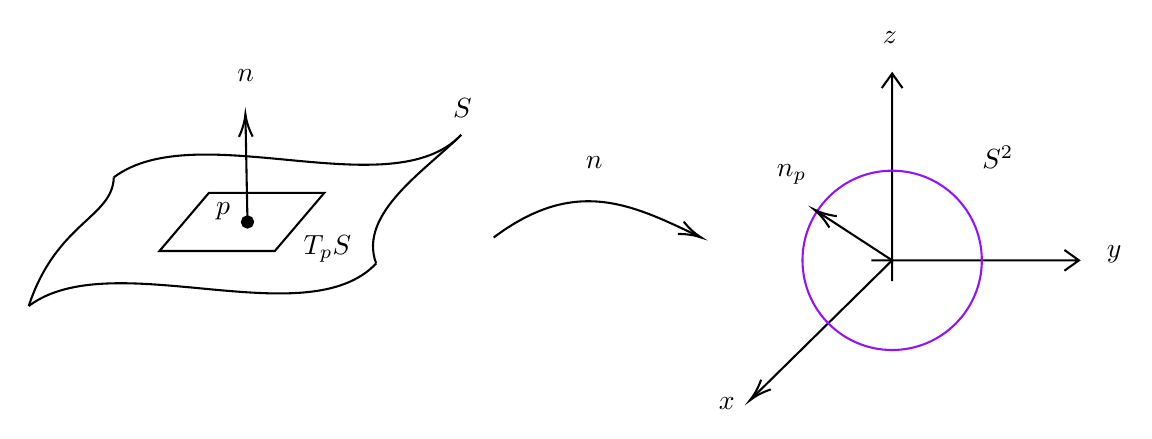
\begin{tikzpicture}[x=0.75pt,y=0.75pt,yscale=-1,xscale=1]
%uncomment if require: \path (0,300); %set diagram left start at 0, and has height of 300

%Curve Lines [id:da28129415507356703] 
\draw    (100,110) .. controls (140,80) and (233.8,125) .. (267.4,89.5) ;
%Curve Lines [id:da9562883564686324] 
\draw    (59,172) .. controls (99,142) and (192.8,187) .. (226.4,151.5) ;
%Curve Lines [id:da748577885122705] 
\draw    (59,172) .. controls (72.4,131.5) and (99.4,129.5) .. (100,110) ;
%Curve Lines [id:da2562375766370064] 
\draw    (226.4,151.5) .. controls (217.4,127.5) and (250.4,106.5) .. (267.4,89.5) ;
%Shape: Parallelogram [id:dp8965230202175429] 
\draw   (145.82,117.5) -- (201.4,117.5) -- (177.58,145.5) -- (122,145.5) -- cycle ;
%Shape: Circle [id:dp3509817579048975] 
\draw  [fill={rgb, 255:red, 0; green, 0; blue, 0 }  ,fill opacity=1 ] (161.7,131.5) .. controls (161.7,130.01) and (162.91,128.8) .. (164.4,128.8) .. controls (165.89,128.8) and (167.1,130.01) .. (167.1,131.5) .. controls (167.1,132.99) and (165.89,134.2) .. (164.4,134.2) .. controls (162.91,134.2) and (161.7,132.99) .. (161.7,131.5) -- cycle ;
%Straight Lines [id:da4477857542457926] 
\draw    (164.4,131.5) -- (163.44,81.5) ;
\draw [shift={(163.4,79.5)}, rotate = 88.9] [color={rgb, 255:red, 0; green, 0; blue, 0 }  ][line width=0.75]    (10.93,-3.29) .. controls (6.95,-1.4) and (3.31,-0.3) .. (0,0) .. controls (3.31,0.3) and (6.95,1.4) .. (10.93,3.29)   ;
%Shape: Axis 2D [id:dp2767501351977306] 
\draw  (465,150) -- (565,150)(475,60) -- (475,160) (558,145) -- (565,150) -- (558,155) (470,67) -- (475,60) -- (480,67)  ;
%Straight Lines [id:da9011328855757925] 
\draw    (475,150) -- (407.83,216.1) ;
\draw [shift={(406.4,217.5)}, rotate = 315.46] [color={rgb, 255:red, 0; green, 0; blue, 0 }  ][line width=0.75]    (10.93,-3.29) .. controls (6.95,-1.4) and (3.31,-0.3) .. (0,0) .. controls (3.31,0.3) and (6.95,1.4) .. (10.93,3.29)   ;
%Shape: Circle [id:dp28714049477405257] 
\draw  [color={rgb, 255:red, 144; green, 19; blue, 254 }  ,draw opacity=1 ] (431.8,150) .. controls (431.8,126.14) and (451.14,106.8) .. (475,106.8) .. controls (498.86,106.8) and (518.2,126.14) .. (518.2,150) .. controls (518.2,173.86) and (498.86,193.2) .. (475,193.2) .. controls (451.14,193.2) and (431.8,173.86) .. (431.8,150) -- cycle ;
%Straight Lines [id:da45439583119974114] 
\draw    (475,150) -- (439.08,126.59) ;
\draw [shift={(437.4,125.5)}, rotate = 33.09] [color={rgb, 255:red, 0; green, 0; blue, 0 }  ][line width=0.75]    (10.93,-3.29) .. controls (6.95,-1.4) and (3.31,-0.3) .. (0,0) .. controls (3.31,0.3) and (6.95,1.4) .. (10.93,3.29)   ;
%Curve Lines [id:da1330380081969107] 
\draw    (283,139) .. controls (322.4,109.45) and (349.58,123.08) .. (381.54,138.3) ;
\draw [shift={(383,139)}, rotate = 205.43] [color={rgb, 255:red, 0; green, 0; blue, 0 }  ][line width=0.75]    (10.93,-3.29) .. controls (6.95,-1.4) and (3.31,-0.3) .. (0,0) .. controls (3.31,0.3) and (6.95,1.4) .. (10.93,3.29)   ;

% Text Node
\draw (190,136.4) node [anchor=north west][inner sep=0.75pt]    {$T_{p} S$};
% Text Node
\draw (158,56.4) node [anchor=north west][inner sep=0.75pt]    {$\vb{n}$};
% Text Node
\draw (147.82,120.9) node [anchor=north west][inner sep=0.75pt]    {$p$};
% Text Node
\draw (262,70.4) node [anchor=north west][inner sep=0.75pt]    {$S$};
% Text Node
\draw (390,214.4) node [anchor=north west][inner sep=0.75pt]    {$x$};
% Text Node
\draw (577,141.4) node [anchor=north west][inner sep=0.75pt]    {$y$};
% Text Node
\draw (469,38.4) node [anchor=north west][inner sep=0.75pt]    {$z$};
% Text Node
\draw (517,93.4) node [anchor=north west][inner sep=0.75pt]    {$\mathbb{S}^{2}$};
% Text Node
\draw (418,102.4) node [anchor=north west][inner sep=0.75pt]   {$\vb{n}_{p}$};
% Text Node
\draw (326,98.4) node [anchor=north west][inner sep=0.75pt]    {$\vb{n}$};


\end{tikzpicture}
\end{center}
Let \(\varphi \colon U\to S\) be a local parametrization near 
\(p\in S\), then 
\[
    \vb{n}=\frac{\varphi_u\wedge\varphi_v}{
        \left|\varphi_u\wedge\varphi_v\right|}.    
\]
Let's compute the differential of the Gauss map at \(p\).
\[
    \dd\vb{n}_p\colon T_p S\to T_{\vb{n}_p}\mathbb{S}^2    .
\]
\(\forall v\in T_p S\), let \(\alpha(s)\) be the curve on \(S\)
such that \(\alpha(0)=p\), \(\alpha'(0)=v\).
\[
    \Rightarrow
    \dd\vb{n}_p(v)=\left.\dv{s}\right|_{s=0}\vb{n}\left(\alpha(s)\right)
    (\text{changing rate of the Gauss map at }p
    \text{ along direction }v).
\]
Note \(\left\langle\vb{n}\left(\alpha(s)\right),
\vb{n}\left(\alpha(s)\right)\right\rangle=1\), taking derivation at 
\(s=0\): 
\[
\left\langle\left.\dv{s}\right|_{s=0}\vb{n}\left(\alpha(s)\right),
\vb{n}_p \right\rangle=0.
\]
\[
    \Rightarrow 
    \dd\vb{n}_p(v)=\left.\dv{s}\right|_{s=0}\vb{n}\left(\alpha(s)\right)
    \in T_p S.
\]
\begin{definition}[The \engordnumber{2} fundamental form]
    \hfill
    \begin{itemize}
        \item \(\forall v\in T_p S\), the \engordnumber{2} fundamental
        form 
        \[\II_p(v,v)=
        -\left\langle\dd\vb{n}_p(v),
        v\right\rangle_{\mathbb{R}^3}\footnotemark.\]
        \footnotetext{Thus, \(\dd\vb{n}_p\colon T_p S\to T_p S\) 
        is a linear map, which is the directional derivation of 
        \(\vb{n}\) along a tangent direction of \(S\).}
        \item More generally \(\forall v,w\in T_p S\), 
        \[
            \II_p\colon T_p S\times T_p S\to T_p \mathbb{R}
        \]
         \[   (v,w)\mapsto \II_p(v,w)=-\left\langle
                \dd\vb{n}_p(v),w\right\rangle_{\mathbb{R}^3}.
        \]

    \end{itemize}
    \(-\dd \vb{n}_p\) is also called the shape operator.
\end{definition}
Before we explore \(\II_p\), let's compute the Gauss map's
differential.

\(\bullet\) Let \(\varphi(u,v)\) be a local parametrization. 
Any curve on \(S\) has parametrization
\[  
    \alpha(t)=\varphi\left(u(t),v(t)\right)=
    \left(x\left(u(t),v(t)\right),
        y\left(u(t),v(t)\right),
        z\left(u(t),v(t)\right)\right).
\]
\[\Rightarrow \alpha'(0)=\varphi_u u'(0)+\varphi_v v'(0).\]
\begin{align*}
    \dd \vb{n}_p\left(\alpha'(0)\right)
    &=\left.\dv{t}\right|_{t=0}\vb{n}\left(\alpha(t)\right)\\
    &=\left.\dv{t}\right|_{t=0}\vb{n}
    \left(x\left(u(t),v(t)\right),
        y\left(u(t),v(t)\right),
        z\left(u(t),v(t)\right)\right)\\
    &=\left(\vb{n}_x x_u+\vb{n}_y y_u+\vb{n}_z z_u\right)u'(0)
    +\left(\vb{n}_x x_v+\vb{n}_y y_v+\vb{n}_z z_v\right)v'(0)\\    
    &=\vb{n}_u u'(0)+\vb{n}_v v'(0).
\end{align*}
On the other hand, by the linearity of \(\dd \vb{n}_p\), 
\[
    \dd \vb{n}_p\left(\alpha'(0)\right)=u'(0)\dd \vb{n}_p
    \left(\varphi_u\right)+v'(0)\dd \vb{n}_p \left(\varphi_v\right).    
\]
\[
    \Rightarrow
    \begin{cases}
        \dd \vb{n}_p\left(\vphi_u\right)=\vb{n}_u,\\
        \dd \vb{n}_p\left(\vphi_v\right)=\vb{n}_v.
    \end{cases}
\]
\begin{align*}
    \left\langle\dd \vb{n}_p\left(\vphi_u\right),\vphi_u
    \right\rangle
    &=\left\langle\vb{n}_u,\vphi_u\right\rangle=
    \pdv{u}\underbrace{\left\langle\vb{n},\vphi_u\right\rangle}_{=0}
    -\left\langle\vb{n},\vphi_{uu}\right\rangle\\
    \left\langle\dd \vb{n}_p\left(\vphi_u\right),\vphi_v
    \right\rangle
    &=\left\langle\vb{n}_u,\vphi_v\right\rangle\\
    &=\pdv{u}\underbrace{\left\langle\vb{n},\vphi_v\right\rangle}_{=0}
    -\left\langle\vb{n},\vphi_{vu}\right\rangle\\
    &=-\left\langle\vb{n},\vphi_{vu}\right\rangle\\
    \left\langle\dd \vb{n}_p\left(\vphi_v\right),\vphi_u
    \right\rangle
    &=\left\langle\vb{n}_v,\vphi_u\right\rangle\\
    &=-\left\langle\vb{n},\vphi_{uv}\right\rangle
    (\text{Note that }\vphi_{uv}=\vphi_{vu}\text{ since }
    \vphi\text{ is smooth})\\
    \left\langle\dd \vb{n}_p\left(\vphi_v\right),\vphi_v
    \right\rangle
    &=\left\langle\vb{n}_v,\vphi_v\right\rangle
    =-\left\langle \vb{n}, \vphi_{vv}\right\rangle.
\end{align*}
Hence, we conclude that: 
\begin{theorem}
    \(\II_p(v,w)=\II_p(w,v)\), \ie\ 
    \(\II_p\) is symmetric in \(v\), \(w\), and
    \(\II_p\) is a bilinear form. 
\end{theorem}
\begin{remark}
    \hfill
    \begin{enumerate}[(1)]
        \item From the computation above, we see that 
        \(\dd \vb{n}_p\) is self-adjoint, \ie\ 
        \(\left\langle\dd \vb{n}_p(v),w\right\rangle=
        \left\langle v,\dd \vb{n}_p(w)\right\rangle
        \).
        \item The \engordnumber{2} fundamental form can also be
        defined as 
        \[\II_p(v)=\left\langle\vb{n}_p,\alpha''(0)\right\rangle,\]
        where \(\alpha\) is a curve with \(\alpha'(0)=v\).
    \end{enumerate}
\end{remark}